\begin{center}

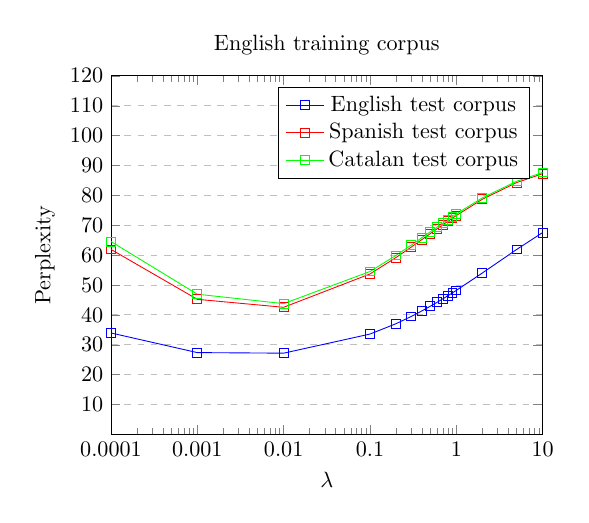
\begin{tikzpicture}[scale=.8]
\begin{semilogxaxis}[
	  log ticks with fixed point,
    title={English training corpus},
    xlabel={$\lambda$},
    ylabel={Perplexity},
    xmin=.0001, xmax=10,
    ymin=0, ymax=120,
    xtick={.0001,.001,.01,.1,1,10},
    ytick={10,20,30,40,50,60,70,80,90,100,110,120},
    legend pos=north east,
    ymajorgrids=true,
    grid style=dashed,
]
 
\addplot[
    color=blue,
    mark=square,
    ]
    coordinates {
(0.00010000,33.9709175258568834)
(0.00100000,27.4005511876346759)
(0.01000000,27.2097439275709441)
(0.10000000,33.5985835905475838)
(0.20000000,37.0677718009028538)
(0.30000000,39.4788092430601907)
(0.40000000,41.3613865129498492)
(0.50000000,42.9165817619826200)
(0.60000000,44.2456519106959192)
(0.70000000,45.4077856958292116)
(0.80000000,46.4409786021626516)
(0.90000000,47.3712514318499558)
(1.00000000,48.2172914439390325)
(2.00000000,54.0290851758192403)
(5.00000000,61.9127302723112507)
(10.00000000,67.5768854086005319)
    };

\addplot[
    color=red,
    mark=square,
    ]
    coordinates {
(0.00010000,61.9293643231486683)
(0.00100000,45.2245332736110939)
(0.01000000,42.5574836721390923)
(0.10000000,53.7101111897372050)
(0.20000000,59.1994413233687524)
(0.30000000,62.6870612303354662)
(0.40000000,65.2315816540894531)
(0.50000000,67.2198384375658122)
(0.60000000,68.8398966326601141)
(0.70000000,70.1982373568702940)
(0.80000000,71.3612447700040917)
(0.90000000,72.3731654469400070)
(1.00000000,73.2649806428615875)
(2.00000000,78.6932003618633900)
(5.00000000,84.2990350925301755)
(10.00000000,87.2566046186265964)
    };

\addplot[
    color=green,
    mark=square,
    ]
    coordinates {
(0.00010000,64.5575648340690549)
(0.00100000,46.9384465764989187)
(0.01000000,43.7812853518558356)
(0.10000000,54.5361862645400990)
(0.20000000,59.9229150217624067)
(0.30000000,63.3570577046293764)
(0.40000000,65.8667623724476385)
(0.50000000,67.8298274646582655)
(0.60000000,69.4304791565654824)
(0.70000000,70.7732314016364938)
(0.80000000,71.9233347272253241)
(0.90000000,72.9243274319720314)
(1.00000000,73.8067212681013416)
(2.00000000,79.1807565363579045)
(5.00000000,84.7333102332676589)
(10.00000000,87.6636747088140567)
    };
    \legend{English test corpus,Spanish test corpus,Catalan test corpus}
 
\end{semilogxaxis}
\end{tikzpicture}
\qquad
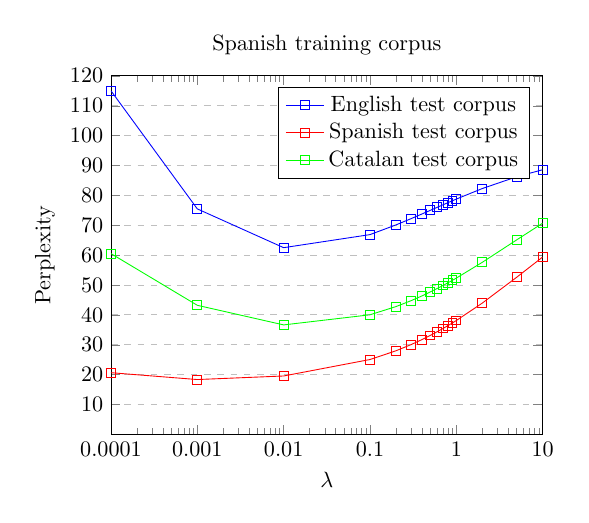
\begin{tikzpicture}[scale=.8]
\begin{semilogxaxis}[
	  log ticks with fixed point,
    title={Spanish training corpus},
    xlabel={$\lambda$},
    ylabel={Perplexity},
    xmin=.0001, xmax=10,
    ymin=0, ymax=120,
    xtick={.0001,.001,.01,.1,1,10},
    ytick={10,20,30,40,50,60,70,80,90,100,110,120},
    legend pos=north east,
    ymajorgrids=true,
    grid style=dashed,
]
 
\addplot[
    color=blue,
    mark=square,
    ]
    coordinates {
(0.00010000,115.0053619565369729)
(0.00100000,75.4853887104112289)
(0.01000000,62.5052614797095600)
(0.10000000,66.8762493662645312)
(0.20000000,70.1252654457947102)
(0.30000000,72.2317168551112729)
(0.40000000,73.7820928246359955)
(0.50000000,75.0017082979238410)
(0.60000000,76.0016187563071526)
(0.70000000,76.8450289737452295)
(0.80000000,77.5714297999730178)
(0.90000000,78.2071695995993821)
(1.00000000,78.7707074594325150)
(2.00000000,82.2934524436399784)
(5.00000000,86.2373777057487416)
(10.00000000,88.5788224852972093)
    };

\addplot[
    color=red,
    mark=square,
    ]
    coordinates {
		(0.00010000,20.6760031479876538)
(0.00100000,18.3840827716670603)
(0.01000000,19.5767372417079635)
(0.10000000,25.0854466667628841)
(0.20000000,28.0077074037100573)
(0.30000000,30.0929036594315171)
(0.40000000,31.7584906104060885)
(0.50000000,33.1611175396782230)
(0.60000000,34.3798112240092379)
(0.70000000,35.4610346149883569)
(0.80000000,36.4348314732418146)
(0.90000000,37.3219375810710758)
(1.00000000,38.1373623781581585)
(2.00000000,43.9724864478504571)
(5.00000000,52.6044758717082743)
(10.00000000,59.3879363348696714)
    };

\addplot[
    color=green,
    mark=square,
    ]
    coordinates {
    (0.00010000,60.5286457523718013)
(0.00100000,43.2242857890149210)
(0.01000000,36.6650279026207997)
(0.10000000,40.0463942016478853)
(0.20000000,42.7977610985461681)
(0.30000000,44.7850729495982378)
(0.40000000,46.3679430611565309)
(0.50000000,47.6938928358624352)
(0.60000000,48.8395240144913316)
(0.70000000,49.8504318750986641)
(0.80000000,50.7562635173611127)
(0.90000000,51.5775269152549143)
(1.00000000,52.3290730155653563)
(2.00000000,57.6114754158890179)
(5.00000000,65.1107296243359599)
(10.00000000,70.7124119486652205)
    };
    \legend{English test corpus,Spanish test corpus,Catalan test corpus}
 
\end{semilogxaxis}
\end{tikzpicture}

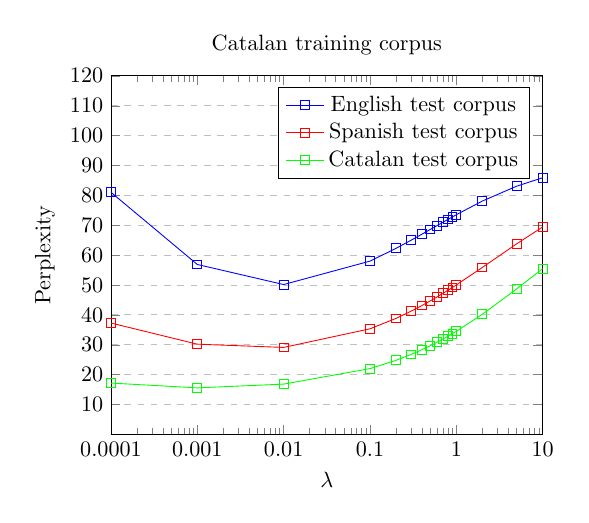
\begin{tikzpicture}[scale=.8]
\begin{semilogxaxis}[
	  log ticks with fixed point,
    title={Catalan training corpus},
    xlabel={$\lambda$},
    ylabel={Perplexity},
    xmin=.0001, xmax=10,
    ymin=0, ymax=120,
    xtick={.0001,.001,.01,.1,1,10},
    ytick={10,20,30,40,50,60,70,80,90,100,110,120},
    legend pos=north east,
    ymajorgrids=true,
    grid style=dashed,
]
 
\addplot[
    color=blue,
    mark=square,
    ]
    coordinates {
    (0.00010000,81.0364047755355870)
(0.00100000,56.8886418281901101)
(0.01000000,50.1662482730151353)
(0.10000000,58.0033848104038228)
(0.20000000,62.2733261742239890)
(0.30000000,65.0125940224562129)
(0.40000000,67.0276174394913511)
(0.50000000,68.6144452022617486)
(0.60000000,69.9169402688004453)
(0.70000000,71.0165552173472747)
(0.80000000,71.9641155871098874)
(0.90000000,72.7935537758674940)
(1.00000000,73.5286816446798355)
(2.00000000,78.1038675737968617)
(5.00000000,83.0883677773916105)
(10.00000000,85.9021779016435545)
    };

\addplot[
    color=red,
    mark=square,
    ]
    coordinates {
    (0.00010000,37.2923115076113945)
(0.00100000,30.2193378967271187)
(0.01000000,29.1309249874060079)
(0.10000000,35.3588271770579823)
(0.20000000,38.8451628287614241)
(0.30000000,41.2653338053674332)
(0.40000000,43.1547831949269067)
(0.50000000,44.7160924137469280)
(0.60000000,46.0509041114217936)
(0.70000000,47.2184977677255304)
(0.80000000,48.2568817992484540)
(0.90000000,49.1920736374679635)
(1.00000000,50.0427579461929355)
(2.00000000,55.8876277313358969)
(5.00000000,63.7974405749786939)
(10.00000000,69.4387859495200814)
    };

\addplot[
    color=green,
    mark=square,
    ]
    coordinates {
    (0.00010000,17.2084235331928639)
(0.00100000,15.6006642684765620)
(0.01000000,16.8531838906264646)
(0.10000000,22.0439732506697013)
(0.20000000,24.8093680467999462)
(0.30000000,26.7930409864643089)
(0.40000000,28.3837506955428900)
(0.50000000,29.7274825109718961)
(0.60000000,30.8980143297787393)
(0.70000000,31.9388042815704694)
(0.80000000,32.8780032012281040)
(0.90000000,33.7350726162849952)
(1.00000000,34.5241212835404525)
(2.00000000,40.2043805187960501)
(5.00000000,48.7166922836574088)
(10.00000000,55.5054185149308594)
    };
    \legend{English test corpus,Spanish test corpus,Catalan test corpus}
 
\end{semilogxaxis}
\end{tikzpicture}

\end{center}